\chapter{Fundamental Concepts}\label{svn.basic}

This chapter is a short, casual introduction to Subversion and its
approach to version control. We begin with a discussion of general
version control concepts, work our way into the specific ideas behind
Subversion, and show some simple examples of Subversion in use.

Even though the examples in this chapter show people sharing collections
of program source code, keep in mind that Subversion can manage any sort
of file collection---it\textquotesingle s not limited to helping
computer programmers.

\section{Version Control Basics}\label{svn.basic.version-control-basics}

A version control system (or revision control system) is a system that
tracks incremental versions (or revisions) of files and, in some cases,
directories over time. Of course, merely tracking the various versions
of a user\textquotesingle s (or group of users\textquotesingle) files
and directories isn\textquotesingle t very interesting in itself. What
makes a version control system useful is the fact that it allows you to
explore the changes which resulted in each of those versions and
facilitates the arbitrary recall of the same.

In this section, we\textquotesingle ll introduce some fairly high-level
version control system components and concepts. We\textquotesingle ll
limit our discussion to modern version control systems---in
today\textquotesingle s interconnected world, there is very little point
in acknowledging version control systems which cannot operate across
wide-area networks.

\subsection{The Repository}\label{svn.basic.repository}

At the core of the version control system is a repository, which is the
central store of that system\textquotesingle s data. The repository
usually stores information in the form of a filesystem tree---a
hierarchy of files and directories. Any number of clients connect to the
repository, and then read or write to these files. By writing data, a
client makes the information available to others; by reading data, the
client receives information from others.
\hyperref[svn.basic.repository.dia-1]{A typical client/server system}
illustrates this.

\begin{figure}
\centering
\pandocbounded{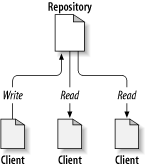
\includegraphics[keepaspectratio]{images/ch02dia1.png}}
\caption{A typical client/server
system}\label{svn.basic.repository.dia-1}
\end{figure}

Why is this interesting? So far, this sounds like the definition of a
typical file server. And indeed, the repository \emph{is} a kind of file
server, but it\textquotesingle s not your usual breed. What makes the
repository special is that as the files in the repository are changed,
the repository remembers each version of those files.

When a client reads data from the repository, it normally sees only the
latest version of the filesystem tree. But what makes a version control
client interesting is that it also has the ability to request previous
states of the filesystem from the repository. A version control client
can ask historical questions such as ``What did this directory contain
last Wednesday?'' and ``Who was the last person to change this file, and
what changes did he make?'' These are the sorts of questions that are at
the heart of any version control system.

\subsection{The Working Copy}\label{svn.basic.working-copy}

A version control system\textquotesingle s value comes from the fact
that it tracks versions of files and directories, but the rest of the
software universe doesn\textquotesingle t operate on ``versions of files
and directories''. Most software programs understand how to operate only
on a \emph{single} version of a specific type of file. So how does a
version control user interact with an abstract---and, often,
remote---repository full of multiple versions of various files in a
concrete fashion? How does his or her word processing software,
presentation software, source code editor, web design software, or some
other program---all of which trade in the currency of simple data
files---get access to such files? The answer is found in the version
control construct known as a working copy.

A working copy is, quite literally, a local copy of a particular version
of a user\textquotesingle s VCS-managed data upon which that user is
free to work. Working copies\footnote{The term ``working copy'' can be
  generally applied to any one file version\textquotesingle s local
  instance. When most folks use the term, though, they are referring to
  a whole directory tree containing files and subdirectories managed by
  the version control system.} appear to other software just as any
other local directory full of files, so those programs
don\textquotesingle t have to be ``version-control-aware'' in order to
read from and write to that data. The task of managing the working copy
and communicating changes made to its contents to and from the
repository falls squarely to the version control
system\textquotesingle s client software.

\subsection{Versioning Models}\label{svn.basic.vsn-models}

If the primary mission of a version control system is to track the
various versions of digital information over time, a very close
secondary mission in any modern version control system is to enable
collaborative editing and sharing of that data. But different systems
use different strategies to achieve this. It\textquotesingle s important
to understand these different strategies, for a couple of reasons.
First, it will help you compare and contrast existing version control
systems, in case you encounter other systems similar to Subversion.
Beyond that, it will also help you make more effective use of
Subversion, since Subversion itself supports a couple of different ways
of working.

\subsubsection{The problem of file
sharing}\label{svn.basic.vsn-models.problem-sharing}

All version control systems have to solve the same fundamental problem:
how will the system allow users to share information, but prevent them
from accidentally stepping on each other\textquotesingle s feet?
It\textquotesingle s all too easy for users to accidentally overwrite
each other\textquotesingle s changes in the repository.

Consider the scenario shown in
\hyperref[svn.basic.vsn-models.problem-sharing.dia-1]{The problem to
avoid}. Suppose we have two coworkers, Harry and Sally. They each decide
to edit the same repository file at the same time. If Harry saves his
changes to the repository first, it\textquotesingle s possible that (a
few moments later) Sally could accidentally overwrite them with her own
new version of the file. While Harry\textquotesingle s version of the
file won\textquotesingle t be lost forever (because the system remembers
every change), any changes Harry made \emph{won\textquotesingle t} be
present in Sally\textquotesingle s newer version of the file, because
she never saw Harry\textquotesingle s changes to begin with.
Harry\textquotesingle s work is still effectively lost---or at least
missing from the latest version of the file---and probably by accident.
This is definitely a situation we want to avoid!

\begin{figure}
\centering
\pandocbounded{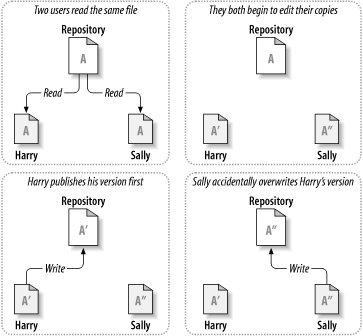
\includegraphics[keepaspectratio]{images/ch02dia2.png}}
\caption{The problem to
avoid}\label{svn.basic.vsn-models.problem-sharing.dia-1}
\end{figure}

\subsubsection{The lock-modify-unlock
solution}\label{svn.basic.vsn-models.lock-unlock}

Many version control systems use a lock-modify-unlock model to address
the problem of many authors clobbering each other\textquotesingle s
work. In this model, the repository allows only one person to change a
file at a time. This exclusivity policy is managed using locks. Harry
must ``lock'' a file before he can begin making changes to it. If Harry
has locked a file, Sally cannot also lock it, and therefore cannot make
any changes to that file. All she can do is wait for Harry to finish his
changes, save the file and release his lock. After Harry unlocks the
file, Sally can take her turn by locking the file. Then she may read the
latest version of the file and edit it.
\hyperref[svn.basic.vsn-models.lock-unlock.dia-1]{The lock-modify-unlock
solution} demonstrates this simple solution.

\begin{figure}
\centering
\pandocbounded{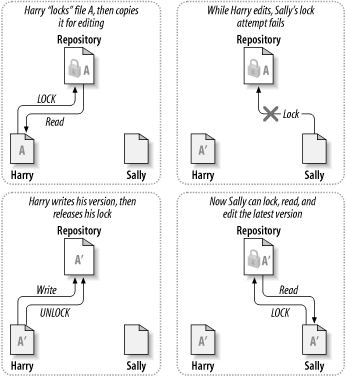
\includegraphics[keepaspectratio]{images/ch02dia3.png}}
\caption{The lock-modify-unlock
solution}\label{svn.basic.vsn-models.lock-unlock.dia-1}
\end{figure}

The problem with the lock-modify-unlock model is that
it\textquotesingle s a bit restrictive and often becomes a roadblock for
users:

\begin{itemize}
\item
  \emph{Locking may cause administrative problems.} Sometimes Harry will
  lock a file and then forget about it. Meanwhile, because Sally is
  still waiting to edit the file, her hands are tied. And then Harry
  goes on vacation. Now Sally has to get an administrator to release
  Harry\textquotesingle s lock. The situation ends up causing a lot of
  unnecessary delay and wasted time.
\item
  \emph{Locking may cause unnecessary serialization.} What if Harry is
  editing the beginning of a text file, and Sally simply wants to edit
  the end of the same file? These changes don\textquotesingle t overlap
  at all. They could easily edit the file simultaneously, and no great
  harm would come, assuming the changes were properly merged together.
  There\textquotesingle s no need for them to take turns in this
  situation.
\item
  \emph{Locking may create a false sense of security.} Suppose Harry
  locks and edits file A, while Sally simultaneously locks and edits
  file B. But what if A and B depend on one another, and the changes
  made to each are semantically incompatible? Suddenly A and B
  don\textquotesingle t work together anymore. The locking system was
  powerless to prevent the problem---yet it somehow provided a false
  sense of security. It\textquotesingle s easy for Harry and Sally to
  imagine that by locking files, each is beginning a safe, insulated
  task, and thus they need not bother discussing their incompatible
  changes early on. Locking often becomes a substitute for real
  communication.
\end{itemize}

\subsubsection{The copy-modify-merge
solution}\label{svn.basic.vsn-models.copy-merge}

Subversion, CVS, and many other version control systems use a
copy-modify-merge model as an alternative to locking. In this model,
each user\textquotesingle s client contacts the project repository and
creates a personal working copy. Users then work simultaneously and
independently, modifying their private copies. Finally, the private
copies are merged together into a new, final version. The version
control system often assists with the merging, but ultimately, a human
being is responsible for making it happen correctly.

Here\textquotesingle s an example. Say that Harry and Sally each create
working copies of the same project, copied from the repository. They
work concurrently and make changes to the same file A within their
copies. Sally saves her changes to the repository first. When Harry
attempts to save his changes later, the repository informs him that his
file A is out of date. In other words, file A in the repository has
somehow changed since he last copied it. So Harry asks his client to
merge any new changes from the repository into his working copy of file
A. Chances are that Sally\textquotesingle s changes
don\textquotesingle t overlap with his own; once he has both sets of
changes integrated, he saves his working copy back to the repository.
\hyperref[svn.basic.vsn-models.copy-merge.dia-1]{The copy-modify-merge
solution} and \hyperref[svn.basic.vsn-models.copy-merge.dia-2]{The
copy-modify-merge solution (continued)} show this process.

\begin{figure}
\centering
\pandocbounded{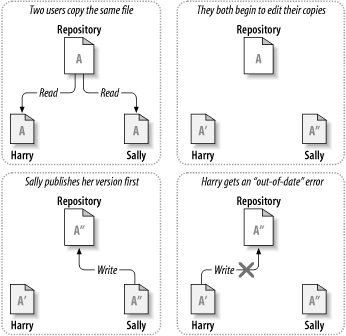
\includegraphics[keepaspectratio]{images/ch02dia4.png}}
\caption{The copy-modify-merge
solution}\label{svn.basic.vsn-models.copy-merge.dia-1}
\end{figure}

\begin{figure}
\centering
\pandocbounded{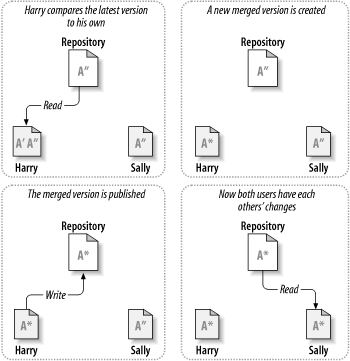
\includegraphics[keepaspectratio]{images/ch02dia5.png}}
\caption{The copy-modify-merge solution
(continued)}\label{svn.basic.vsn-models.copy-merge.dia-2}
\end{figure}

But what if Sally\textquotesingle s changes \emph{do} overlap with
Harry\textquotesingle s changes? What then? This situation is called a
conflict, and it\textquotesingle s usually not much of a problem. When
Harry asks his client to merge the latest repository changes into his
working copy, his copy of file A is somehow flagged as being in a state
of conflict: he\textquotesingle ll be able to see both sets of
conflicting changes and manually choose between them. Note that software
can\textquotesingle t automatically resolve conflicts; only humans are
capable of understanding and making the necessary intelligent choices.
Once Harry has manually resolved the overlapping changes---perhaps after
a discussion with Sally---he can safely save the merged file back to the
repository.

The copy-modify-merge model may sound a bit chaotic, but in practice, it
runs extremely smoothly. Users can work in parallel, never waiting for
one another. When they work on the same files, it turns out that most of
their concurrent changes don\textquotesingle t overlap at all; conflicts
are infrequent. And the amount of time it takes to resolve conflicts is
usually far less than the time lost by a locking system.

In the end, it all comes down to one critical factor: user
communication. When users communicate poorly, both syntactic and
semantic conflicts increase. No system can force users to communicate
perfectly, and no system can detect semantic conflicts. So
there\textquotesingle s no point in being lulled into a false sense of
security that a locking system will somehow prevent conflicts; in
practice, locking seems to inhibit productivity more than anything else.

\protect\phantomsection\label{svn.basic.vsn-models.copy-merge.sb-1}
When Locking Is Necessary

While the lock-modify-unlock model is considered generally harmful to
collaboration, sometimes locking is appropriate.

The copy-modify-merge model is based on the assumption that files are
contextually mergeable---that is, that the majority of the files in the
repository are line-based text files (such as program source code). But
for files with binary formats, such as artwork or sound,
it\textquotesingle s often impossible to merge conflicting changes. In
these situations, it really is necessary for users to take strict turns
when changing the file. Without serialized access, somebody ends up
wasting time on changes that are ultimately discarded.

While Subversion is primarily a copy-modify-merge system, it still
recognizes the need to lock an occasional file, and thus provides
mechanisms for this. We discuss this feature in
\hyperref[svn.advanced.locking]{Locking}.

\section{Version Control the Subversion Way}\label{svn.basic.in-action}

We\textquotesingle ve mentioned already that Subversion is a modern,
network-aware version control system. As we described in
\hyperref[svn.basic.version-control-basics]{Version Control Basics} (our
high-level version control overview), a repository serves as the core
storage mechanism for Subversion\textquotesingle s versioned data, and
it\textquotesingle s via working copies that users and their software
programs interact with that data. In this section, we\textquotesingle ll
begin to introduce the specific ways in which Subversion implements
version control.

\subsection{Subversion Repositories}\label{svn.basic.svn-repositories}

Subversion implements the concept of a version control repository much
as any other modern version control system would. Unlike a working copy,
a Subversion repository is an abstract entity, able to be operated upon
almost exclusively by Subversion\textquotesingle s own libraries and
tools. As most of a user\textquotesingle s Subversion interactions
involve the use of the Subversion client and occur in the context of a
working copy, we spend the majority of this book discussing the
Subversion working copy and how to manipulate it. For the finer details
of the repository, though, check out
\hyperref[svn.reposadmin]{Repository Administration}.

\protect\phantomsection\label{svn.basic.svn-repositories.not-working-copy}
In Subversion, the client-side object which every user of the system
has---the directory of versioned files, along with metadata that enables
the system to track them and communicate with the server---is called a
\emph{working copy}. Although other version control systems use the term
``repository'' for the client-side object, it is both incorrect and a
common source of confusion to use the term in that way in the context of
Subversion.

Working copies are described later, in
\hyperref[svn.basic.in-action.wc]{Subversion Working Copies}.

\subsection{Revisions}\label{svn.basic.in-action.revs}

A Subversion client commits (that is, communicates the changes made to)
any number of files and directories as a single atomic transaction. By
atomic transaction, we mean simply this: either all of the changes are
accepted into the repository, or none of them is. Subversion tries to
retain this atomicity in the face of program crashes, system crashes,
network problems, and other users\textquotesingle{} actions.

Each time the repository accepts a commit, this creates a new state of
the filesystem tree, called a revision. Each revision is assigned a
unique natural number, one greater than the number assigned to the
previous revision. The initial revision of a freshly created repository
is numbered 0 and consists of nothing but an empty root directory.

\hyperref[svn.basic.in-action.revs.dia-1]{Tree changes over time}
illustrates a nice way to visualize the repository. Imagine an array of
revision numbers, starting at 0, stretching from left to right. Each
revision number has a filesystem tree hanging below it, and each tree is
a ``snapshot'' of the way the repository looked after a commit.

\begin{figure}
\centering
\pandocbounded{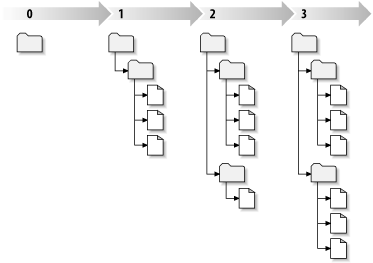
\includegraphics[keepaspectratio]{images/ch02dia7.png}}
\caption{Tree changes over time}\label{svn.basic.in-action.revs.dia-1}
\end{figure}

Global Revision Numbers

Unlike most version control systems, Subversion\textquotesingle s
revision numbers apply to \emph{the entire repository tree}, not
individual files. Each revision number selects an entire tree, a
particular state of the repository after some committed change. Another
way to think about it is that revision N represents the state of the
repository filesystem after the Nth commit. When Subversion users talk
about ``revision 5 of \texttt{foo.c},'' they really mean
``\texttt{foo.c} as it appears in revision 5.'' Notice that in general,
revisions N and M of a file do \emph{not} necessarily differ! Many other
version control systems use per-file revision numbers, so this concept
may seem unusual at first. (Former CVS users might want to see
\hyperref[svn.forcvs]{Subversion for CVS Users} for more details.)

\subsection{Addressing the Repository}\label{svn.advanced.reposurls}

Subversion client programs use URLs to identify versioned files and
directories in Subversion repositories. For the most part, these URLs
use the standard syntax, allowing for server names and port numbers to
be specified as part of the URL.

\begin{itemize}
\tightlist
\item
  http://svn.example.com/svn/project
\item
  http://svn.example.com:9834/repos
\end{itemize}

Subversion repository URLs aren\textquotesingle t limited to only the
\texttt{http://} variety. Because Subversion offers several different
ways for its clients to communicate with its servers, the URLs used to
address the repository differ subtly depending on which repository
access mechanism is employed.
\hyperref[svn.basic.in-action.wc.tbl-1]{Repository access URLs}
describes how different URL schemes map to the available repository
access methods. For more details about Subversion\textquotesingle s
server options, see \hyperref[svn.serverconfig]{Server Configuration}.

\begin{longtable}[]{@{}>{\raggedright\arraybackslash}p{\dimexpr(\linewidth-2\tabcolsep*2)/2\relax}>{\raggedright\arraybackslash}p{\dimexpr(\linewidth-2\tabcolsep*2)/2\relax}@{}}
\caption{Repository access
URLs}\label{svn.basic.in-action.wc.tbl-1}\tabularnewline
\toprule\noalign{}
Schema & Access method \\
\midrule\noalign{}
\endfirsthead
\toprule\noalign{}
Schema & Access method \\
\midrule\noalign{}
\endhead
\bottomrule\noalign{}
\endlastfoot
\texttt{file:///} & Direct repository access (on local disk) \\
\texttt{http://} & Access via WebDAV protocol to Subversion-aware Apache
server \\
\texttt{https://} & Same as \texttt{http://}, but with SSL encapsulation
(encryption and authentication) \\
\texttt{svn://} & Access via custom protocol to an \texttt{svnserve}
server \\
\texttt{svn+ssh://} & Same as \texttt{svn://}, but through an SSH
tunnel \\
\end{longtable}

Subversion\textquotesingle s handling of URLs has some noteworthy
nuances. For example, URLs containing the \texttt{file://} access method
(used for local repositories) must, in accordance with convention, have
either a server name of \texttt{localhost} or no server name at all:

\begin{itemize}
\tightlist
\item
  file:///var/svn/repos
\item
  file://localhost/var/svn/repos
\end{itemize}

Also, users of the \texttt{file://} scheme on Windows platforms will
need to use an unofficially ``standard'' syntax for accessing
repositories that are on the same machine, but on a different drive than
the client\textquotesingle s current working drive. Either of the two
following URL path syntaxes will work, where \texttt{X} is the drive on
which the repository resides:

\begin{itemize}
\tightlist
\item
  file:///X:/var/svn/repos
\item
  file:///X\textbar/var/svn/repos
\end{itemize}

Note that a URL uses forward slashes even though the native (non-URL)
form of a path on Windows uses backslashes. Also note that when using
the \texttt{file:///X\textbar{}/} form at the command line, you need to
quote the URL (wrap it in quotation marks) so that the vertical bar
character is not interpreted as a pipe.

You cannot use Subversion\textquotesingle s \texttt{file://} URLs in a
regular web browser the way you can use typical \texttt{file://} URLs.
When you attempt to view a \texttt{file://} URL in a regular web
browser, it reads and displays the contents of the file at that location
by examining the filesystem directly. However,
Subversion\textquotesingle s resources exist in a virtual filesystem
(see \hyperref[svn.developer.layerlib.repos]{Repository Layer}), and
your browser will not understand how to interact with that filesystem.

The Subversion client will automatically encode URLs as necessary, just
like a web browser does. For example, the URL
\texttt{http://host/path\ with\ space/project/españa} --- which contains
both spaces and upper-ASCII characters --- will be automatically
interpreted by Subversion as if you\textquotesingle d provided
\texttt{http://host/path\%20with\%20space/project/espa\%C3\%B1a}. If the
URL contains spaces, be sure to place it within quotation marks at the
command line so that your shell treats the whole thing as a single
argument to the program.

There is one notable exception to Subversion\textquotesingle s handling
of URLs which also applies to its handling of local paths in many
contexts, too. If the final path component of your URL or local path
contains an at sign (\texttt{@}), you need to use a special
syntax---described in \hyperref[svn.advanced.pegrevs]{Peg and Operative
Revisions}---in order to make Subversion properly address that resource.

In Subversion 1.6, a new caret (\texttt{\^{}}) notation was introduced
as a shorthand for ``the URL of the repository\textquotesingle s root
directory''. For example, you can use the
\texttt{\^{}/tags/bigsandwich/} to refer to the URL of the
\texttt{/tags/bigsandwich} directory in the root of the repository. Such
a URL is called a repository-relative URL. Note that this URL syntax
works only when your current working directory is a working copy---the
command-line client knows the repository\textquotesingle s root URL by
looking at the working copy\textquotesingle s metadata. Also note that
when you wish to refer precisely to the root directory of the
repository, you must do so using \texttt{\^{}/} (with the trailing slash
character), not merely \texttt{\^{}}. Windows users should not forget
that a caret is an escape character on their platform. Therefore, use a
double caret \texttt{\^{}\^{}} if you run the Subversion client on a
Windows machine.

\subsection{Subversion Working Copies}\label{svn.basic.in-action.wc}

A Subversion working copy is an ordinary directory tree on your local
system, containing a collection of files. You can edit these files
however you wish, and if they\textquotesingle re source code files, you
can compile your program from them in the usual way. Your working copy
is your own private work area: Subversion will never incorporate other
people\textquotesingle s changes, nor make your own changes available to
others, until you explicitly tell it to do so. You can even have
multiple working copies of the same project.

After you\textquotesingle ve made some changes to the files in your
working copy and verified that they work properly, Subversion provides
you with commands to ``publish'' your changes (by writing to the
repository), thereby making them available to the other people working
with you on your project. If other people publish their own changes,
Subversion provides you with commands to merge those changes into your
own working copy (by reading from the repository). Notice that the
central repository is the broker for everybody\textquotesingle s changes
in Subversion---changes aren\textquotesingle t passed directly from
working copy to working copy in the typical workflow.

A working copy also contains some extra files, created and maintained by
Subversion, to help it carry out these commands. In particular, each
working copy contains a subdirectory named \texttt{.svn}, also known as
the working copy\textquotesingle s administrative directory. The files
in the administrative directory help Subversion recognize which of your
versioned files contain unpublished changes, and which files are out of
date with respect to others\textquotesingle{} work.

Prior to version 1.7, Subversion maintained \texttt{.svn} administrative
subdirectories in \emph{every} versioned directory of your working copy.
Subversion 1.7 offers a completely new approach to how working copy
metadata is stored and maintained, and chief among the visible changes
to this approach is that each working copy now has only one
\texttt{.svn} subdirectory which is an immediate child of the root of
that working copy.

\subsubsection{How the working copy
works}\label{svn.basic.in-action.track-repos}

For each file in a working directory, Subversion records (among other
things) two essential pieces of information:

\begin{itemize}
\item
  What revision your working file is based on (this is called the
  file\textquotesingle s working revision)
\item
  A timestamp recording when the local copy was last updated by the
  repository
\end{itemize}

Given this information, by talking to the repository, Subversion can
tell which of the following four states a working file is in:

\begin{description}
\item[Unchanged, and current]
The file is unchanged in the working directory, and no changes to that
file have been committed to the repository since its working revision.
An \texttt{svn\ commit} of the file will do nothing, and an
\texttt{svn\ update} of the file will do nothing.
\item[Locally changed, and current]
The file has been changed in the working directory, and no changes to
that file have been committed to the repository since you last updated.
There are local changes that have not been committed to the repository;
thus an \texttt{svn\ commit} of the file will succeed in publishing your
changes, and an \texttt{svn\ update} of the file will do nothing.
\item[Unchanged, and out of date]
The file has not been changed in the working directory, but it has been
changed in the repository. The file should eventually be updated in
order to make it current with the latest public revision. An
\texttt{svn\ commit} of the file will do nothing, and an
\texttt{svn\ update} of the file will fold the latest changes into your
working copy.
\item[Locally changed, and out of date]
The file has been changed both in the working directory and in the
repository. An \texttt{svn\ commit} of the file will fail with an
``out-of-date'' error. The file should be updated first; an
\texttt{svn\ update} command will attempt to merge the public changes
with the local changes. If Subversion can\textquotesingle t complete the
merge in a plausible way automatically, it leaves it to the user to
resolve the conflict.
\end{description}

\subsubsection{Fundamental working copy
interactions}\label{svn.basic.in-action.wc-funcdamentals}

A typical Subversion repository often holds the files (or source code)
for several projects; usually, each project is a subdirectory in the
repository\textquotesingle s filesystem tree. In this arrangement, a
user\textquotesingle s working copy will usually correspond to a
particular subtree of the repository.

For example, suppose you have a repository that contains two software
projects, \texttt{paint} and \texttt{calc}. Each project lives in its
own top-level subdirectory, as shown in
\hyperref[svn.basic.in-action.wc.dia-1]{The repository\textquotesingle s
filesystem}.

\begin{figure}
\centering
\pandocbounded{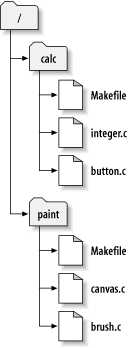
\includegraphics[keepaspectratio]{images/ch02dia6.png}}
\caption{The repository\textquotesingle s
filesystem}\label{svn.basic.in-action.wc.dia-1}
\end{figure}

To get a working copy, you must check out some subtree of the
repository. (The term \emph{check out} may sound like it has something
to do with locking or reserving resources, but it
doesn\textquotesingle t; it simply creates a working copy of the project
for you.) For example, if you check out \texttt{/calc}, you will get a
working copy like this:

\begin{verbatim}
$ svn checkout http://svn.example.com/repos/calc
A    calc/Makefile
A    calc/integer.c
A    calc/button.c
Checked out revision 56.
$ ls -A calc
Makefile  button.c integer.c .svn/
$
\end{verbatim}

The list of letter \texttt{A}s in the left margin indicates that
Subversion is adding a number of items to your working copy. You now
have a personal copy of the repository\textquotesingle s \texttt{/calc}
directory, with one additional entry---\texttt{.svn}---which holds the
extra information needed by Subversion, as mentioned earlier.

Suppose you make changes to \texttt{button.c}. Since the \texttt{.svn}
directory remembers the file\textquotesingle s original modification
date and contents, Subversion can tell that you\textquotesingle ve
changed the file. However, Subversion does not make your changes public
until you explicitly tell it to. The act of publishing your changes is
more commonly known as committing (or checking in) changes to the
repository.

To publish your changes, you can use Subversion\textquotesingle s
\texttt{svn\ commit} command:

\begin{verbatim}
$ svn commit button.c -m "Fixed a typo in button.c."
Sending        button.c
Transmitting file data .
Committed revision 57.
$
\end{verbatim}

Now your changes to \texttt{button.c} have been committed to the
repository, with a note describing your change (namely, that you fixed a
typo). If another user checks out a working copy of \texttt{/calc}, she
will see your changes in the latest version of the file.

Suppose you have a collaborator, Sally, who checked out a working copy
of \texttt{/calc} at the same time you did. When you commit your change
to \texttt{button.c}, Sally\textquotesingle s working copy is left
unchanged; Subversion modifies working copies only at the
user\textquotesingle s request.

To bring her project up to date, Sally can ask Subversion to update her
working copy, by using the \texttt{svn\ update} command. This will
incorporate your changes into her working copy, as well as any others
that have been committed since she checked it out.

\begin{verbatim}
$ pwd
/home/sally/calc
$ ls -A
Makefile button.c integer.c .svn/
$ svn update
Updating '.':
U    button.c
Updated to revision 57.
$
\end{verbatim}

The output from the \texttt{svn\ update} command indicates that
Subversion updated the contents of \texttt{button.c}. Note that Sally
didn\textquotesingle t need to specify which files to update; Subversion
uses the information in the \texttt{.svn} directory as well as further
information in the repository, to decide which files need to be brought
up to date.

\subsubsection{Mixed-revision working
copies}\label{svn.basic.in-action.mixedrevs}

As a general principle, Subversion tries to be as flexible as possible.
One special kind of flexibility is the ability to have a working copy
containing files and directories with a mix of different working
revision numbers. Subversion working copies do not always correspond to
any single revision in the repository; they may contain files from
several different revisions. For example, suppose you check out a
working copy from a repository whose most recent revision is 4:

\begin{verbatim}
calc/
   Makefile:4
   integer.c:4
   button.c:4
\end{verbatim}

At the moment, this working directory corresponds exactly to revision 4
in the repository. However, suppose you make a change to
\texttt{button.c}, and commit that change. Assuming no other commits
have taken place, your commit will create revision 5 of the repository,
and your working copy will now look like this:

\begin{verbatim}
calc/
   Makefile:4
   integer.c:4
   button.c:5
\end{verbatim}

Suppose that, at this point, Sally commits a change to
\texttt{integer.c}, creating revision 6. If you use \texttt{svn\ update}
to bring your working copy up to date, it will look like this:

\begin{verbatim}
calc/
   Makefile:6
   integer.c:6
   button.c:6
\end{verbatim}

Sally\textquotesingle s change to \texttt{integer.c} will appear in your
working copy, and your change will still be present in
\texttt{button.c}. In this example, the text of \texttt{Makefile} is
identical in revisions 4, 5, and 6, but Subversion will mark your
working copy of \texttt{Makefile} with revision 6 to indicate that it is
still current. So, after you do a clean update at the top of your
working copy, it will generally correspond to exactly one revision in
the repository.

\paragraph{Updates and commits are
separate}\label{svn.basic.in-action.mixedrevs.update-commit}

One of the fundamental rules of Subversion is that a ``push'' action
does not cause a ``pull'' nor vice versa. Just because
you\textquotesingle re ready to submit new changes to the repository
doesn\textquotesingle t mean you\textquotesingle re ready to receive
changes that others have checked in. And if you have new changes still
in progress, \texttt{svn\ update} should gracefully merge repository
changes into your own, rather than forcing you to publish them.

The main side effect of this rule is that it means a working copy has to
do extra bookkeeping to track mixed revisions as well as be tolerant of
the mixture. It\textquotesingle s made more complicated by the fact that
directories themselves are versioned.

For example, suppose you have a working copy entirely at revision 10,
while others have been committing their changes so that the youngest
revision in the repository is now revision 14. You edit the file
\texttt{foo.html} and then perform an \texttt{svn\ commit}, which
creates revision 15 in the repository. After the commit succeeds, many
new users would expect the working copy to be entirely at revision 15,
but that\textquotesingle s not the case! Any number of changes might
have happened in the repository between revisions 10 and 15. The client
knows nothing of those changes in the repository, since you
haven\textquotesingle t yet run \texttt{svn\ update}, and
\texttt{svn\ commit} doesn\textquotesingle t pull down new changes. If,
on the other hand, \texttt{svn\ commit} were to automatically download
the newest changes, it would be possible to set the entire working copy
to revision 15---but then we\textquotesingle d be breaking the
fundamental rule of ``push'' and ``pull'' remaining separate actions.
Therefore, the only safe thing the Subversion client can do is mark the
one file---\texttt{foo.html}---as being at revision 15. The rest of the
working copy remains at revision 10. Only by running
\texttt{svn\ update} can the latest changes be downloaded and the whole
working copy be marked as revision 15.

\paragraph{Mixed revisions are
normal}\label{svn.basic.in-action.mixedrevs.normal}

The fact is, \emph{every time} you run \texttt{svn\ commit} your working
copy ends up with some mixture of revisions. The things you just
committed are marked as having larger working revisions than everything
else. After several commits (with no updates in between), your working
copy will contain a whole mixture of revisions. Even if
you\textquotesingle re the only person using the repository, you will
still see this phenomenon. To examine your mixture of working revisions,
use the \texttt{svn\ status} command with the \texttt{-\/-verbose}
(\texttt{-v}) option (see \hyperref[svn.tour.cycle.examine.status]{See
an overview of your changes} for more information).

Often, new users are completely unaware that their working copy contains
mixed revisions. This can be confusing, because many client commands are
sensitive to the working revision of the item they\textquotesingle re
examining. For example, the \texttt{svn\ log} command is used to display
the history of changes to a file or directory (see
\hyperref[svn.tour.history.log]{Generating a List of Historical
Changes}). When the user invokes this command on a working copy object,
he expects to see the entire history of the object. But if the
object\textquotesingle s working revision is quite old (often because
\texttt{svn\ update} hasn\textquotesingle t been run in a long time),
the history of the \emph{older} version of the object is shown.

\paragraph{Mixed revisions are
useful}\label{svn.basic.in-action.mixedrevs.useful}

If your project is sufficiently complex, you\textquotesingle ll discover
that it\textquotesingle s sometimes nice to forcibly backdate (or update
to a revision older than the one you already have) portions of your
working copy to an earlier revision; you\textquotesingle ll learn how to
do that in \hyperref[svn.tour]{Basic Usage}. Perhaps
you\textquotesingle d like to test an earlier version of a submodule
contained in a subdirectory, or perhaps you\textquotesingle d like to
figure out when a bug first came into existence in a specific file. This
is the ``time machine'' aspect of a version control system---the feature
that allows you to move any portion of your working copy forward and
backward in history.

\paragraph{Mixed revisions have
limitations}\label{svn.basic.in-action.mixedrevs.limits}

However you make use of mixed revisions in your working copy, there are
limitations to this flexibility.

First, you cannot commit the deletion of a file or directory that
isn\textquotesingle t fully up to date. If a newer version of the item
exists in the repository, your attempt to delete will be rejected to
prevent you from accidentally destroying changes you\textquotesingle ve
not yet seen.

Second, you cannot commit a metadata change to a directory unless
it\textquotesingle s fully up to date. You\textquotesingle ll learn
about attaching ``properties'' to items in
\hyperref[svn.advanced]{Advanced Topics}. A directory\textquotesingle s
working revision defines a specific set of entries and properties, and
thus committing a property change to an out-of-date directory may
destroy properties you\textquotesingle ve not yet seen.

Finally, beginning in Subversion 1.7, you cannot by default use a
mixed-revision working copy as the target of a merge operation. (This
new requirement was introduced to prevent common problems which stem
from doing so.)

\section{Summary}\label{svn.basic.summary}

We covered a number of fundamental Subversion concepts in this chapter:

\begin{itemize}
\item
  We introduced the notions of the central repository, the client
  working copy, and the array of repository revision trees.
\item
  We saw some simple examples of how two collaborators can use
  Subversion to publish and receive changes from one another, using the
  ``copy-modify-merge'' model.
\item
  We talked a bit about the way Subversion tracks and manages
  information in a working copy.
\end{itemize}

At this point, you should have a good idea of how Subversion works in
the most general sense. Armed with this knowledge, you should now be
ready to move into the next chapter, which is a detailed tour of
Subversion\textquotesingle s commands and features.

